\documentclass[convert={density=300,outext=.png}]{standalone}
\usepackage{pgf,tikz}
\usetikzlibrary{shapes,arrows,automata,positioning}

\begin{document}
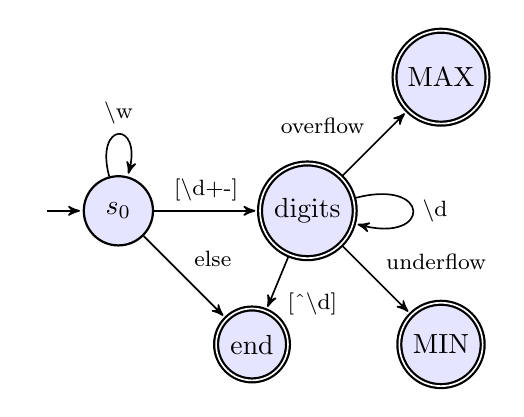
\begin{tikzpicture}[->,>=stealth',shorten >=1pt,auto,node distance=2.4cm,on grid,semithick,every state/.style={fill=blue!10,thick}]
  \node[state,initial,initial text={}] (s0) {$s_0$};
  \node[state,accepting] (digits) [right=of s0] {digits};
  \node[state,accepting] (end) [below right=of s0] {end};
  \node[state,accepting] (overflow) [above right=of digits] {MAX};
  \node[state,accepting] (underflow) [below right=of digits] {MIN};

  \draw[every node/.style={font=\footnotesize}]
  (s0) edge[loop above] node{\textbackslash w} ()
  (s0) edge node{[\textbackslash d+-]} (digits)
  (s0) edge node{else} (end)
  (digits) edge[loop right] node{\textbackslash d} ()
  (digits) edge node{[\string^\textbackslash d]} (end)
  (digits) edge node{overflow} (overflow)
  (digits) edge node{underflow} (underflow)
  ;
\end{tikzpicture}
\end{document}
